\documentclass[12pt,a4paper]{article}

% Langue et encodage
\usepackage[french]{babel}
\usepackage[utf8]{inputenc}
\usepackage[T1]{fontenc}

% TikZ
\usepackage{tikz}
\usetikzlibrary{calc}

% Marges
\usepackage{geometry}
\geometry{margin=1in}



% Couleurs
\usepackage{xcolor}
\definecolor{lightgray}{gray}{0.95}

\usepackage{amsthm}

\newtheorem{lemma}{Lemme}
\newtheorem{theorem}{Théorème}
\newtheorem{corollary}{Corollaire}
\newtheorem{proposition}{Proposition}

\theoremstyle{definition}
\newtheorem{definition}{Définition}

\theoremstyle{remark}
\newtheorem{remark}{Remarque}

% Police machine à écrire propre
\usepackage{courier}
\usepackage{amsmath}
% ======================================================================
%  SUPPORT UTF-8 (pour caractères spéciaux hors minted)
% ======================================================================
\usepackage{newunicodechar}

% Accents français
\newunicodechar{é}{\'e}
\newunicodechar{è}{\`e}
\newunicodechar{ê}{\^e}
\newunicodechar{ë}{\"e}
\newunicodechar{à}{\`a}
\newunicodechar{â}{\^a}
\newunicodechar{ä}{\"a}
\newunicodechar{ù}{\`u}
\newunicodechar{û}{\^u}
\newunicodechar{ü}{\"u}
\newunicodechar{ô}{\^o}
\newunicodechar{î}{\^i}
\newunicodechar{ï}{\"i}
\newunicodechar{ç}{\c{c}}

% Majuscules accentuées
\newunicodechar{É}{\'E}
\newunicodechar{È}{\`E}
\newunicodechar{Ê}{\^E}
\newunicodechar{Ë}{\"E}
\newunicodechar{À}{\`A}
\newunicodechar{Â}{\^A}
\newunicodechar{Ç}{\c{C}}
\newunicodechar{Ô}{\^O}

% Guillemets français
\newunicodechar{<<}{<<}
\newunicodechar{>>}{>>}

% Tirets
\newunicodechar{--}{--}
\newunicodechar{---}{---}

% Symboles mathématiques
\newunicodechar{\\leq }{\leq}
\newunicodechar{\\geq }{\geq}
\newunicodechar{\\neq }{\neq}
\newunicodechar{\\in }{\in}
\newunicodechar{\\notin }{\notin}
\newunicodechar{\\wedge }{\wedge}
\newunicodechar{\\vee }{\vee}
\newunicodechar{\\neg }{\neg}
\newunicodechar{\\forall }{\forall}
\newunicodechar{\\exists }{\exists}
\newunicodechar{\\rightarrow }{\rightarrow}
\newunicodechar{\\Rightarrow }{\Rightarrow}
\newunicodechar{\\leftrightarrow }{\leftrightarrow}
\newunicodechar{\\times }{\times}
\newunicodechar{\\sqrt{}}{\sqrt{}}

% Degré
\newunicodechar{^{\\circ}}{^\circ}

% Espaces invisibles
\newunicodechar{}{}   % ZERO WIDTH SPACE
\newunicodechar{ }{ }  % NARROW NBSP
\newunicodechar{ }{ }  % NBSP

% ======================================================================
%  MINTED --- remplace listings (UTF-8 natif, stable, moderne)
% ======================================================================
\usepackage{minted}
% Option recommandée pour éviter les débordements
\setminted{
    fontsize=\small,
    breaklines=true,
    breakanywhere=true,
    bgcolor=lightgray
}

\begin{document}

\tableofcontents
\clearpage

\begin{titlepage}
    \centering

    {\Huge \textbf{Mecanique harmonique du chaos discret}}\\[1.5cm]

    {\Large \textbf{Auteur :} Philippe Thomas Savard}\\[0.3cm]
    {\large Levis, Chaudiere-Appalaches, Canada}\\[0.8cm]

    {\large \textbf{Licence :} Apache 2.0}\\[0.8cm]

    {\large \textbf{Date :} Le huit mars deux mille vingt-six}\\[2cm]

    \vfill
\end{titlepage}

% ============================================================
% PREFACE
% ============================================================

\vspace{0.5cm}

Ce document a ete redige sans financement, sans avantages materiels ou symboliques, 
et dans une totale liberte de conscience et de jugement. 
Ce texte est le fruit d'une experience de pensee, illustree par des calculs mathematiques, 
des schemas, des tableaux, ainsi que des exemples et explications. 
L'auteur n'est pas initie aux mathematiques au sens academique : 
il ne possede aucune formation specialisee dans ce domaine. 
Il est ouvrier, et c'est en dehors des sentiers balises qu'il a con\c{c}u ce document 
par pur plaisir intellectuel et en consequence d'un interet profond pour les mathematiques.

\vspace{0.5cm}

% ============================================================
% SECTION : FIGURE
% ============================================================

\section{Figure de la mecanique harmonique du chaos discret}

Cette figure est le schema sur lequel l'auteur applique un raisonnement intuitif 
qui lui permet de determiner la possibilite d'une invariance geometrique nouvelle. 
Cette invariance est relative, tout comme la relativite ou la position de l'observateur 
influence la mesure. Dans la mecanique harmonique du chaos discret, 
c'est l'unite choisie qui influence la mesure.

L'auteur trace un parallele avec la constante d'Euler-Mascheroni, 
ou plut\^ot avec l'interet lie a l'exactitude de cette constante, 
qui devient plus precise \`a la quatrieme decimale lorsqu'elle est interpretee 
en sens contraire de la lecture habituelle. 
La constante d'Euler-Mascheroni, qu'il simplifie \`a la forme 
\(0.5 / \sin 60^\circ\), est evoquee dans l'equation lui permettant 
de determiner l'unite. Il emprunte une approche originale pour determiner 
l'unite choisie par le produit du diametre du carre AEFG 
par le rapport entre 0.5 et le resultat de l'arcsin de LM, 
soit : \texttt{AEFG * (0.5 / sin(angle))}.

\vspace{0.8cm}

% ============================================================
% FIGURE TIKZ COMPLETE
% ============================================================

\begin{tikzpicture}[scale=1.8]

% Couleurs
\definecolor{grisA}{gray}{0.55}
\definecolor{grisB}{gray}{0.45}
\definecolor{grisC}{gray}{0.35}

\pgfmathsetmacro{\rtthree}{sqrt(3)}

% Carre principal ABCD (2.25)
\coordinate (A) at (0,0);
\coordinate (B) at (2.25,0);
\coordinate (C) at (2.25,2.25);
\coordinate (D) at (0,2.25);

% Carre interieur AEFG (1.5)
\coordinate (E) at (1.5,0);
\coordinate (F) at (1.5,1.5);
\coordinate (G) at (0,1.5);

% Quadrillage fractal
\foreach \x in {0,0.5,...,2.25}
  \foreach \y in {0,0.5,...,2.25}
    \draw[grisA!70,thin] (\x,\y) rectangle ++(0.5,0.5);

\foreach \x in {0,0.25,...,3.375}
  \foreach \y in {0,0.25,...,3.375}
    {
      \ifdim\x pt<2.25pt
        \ifdim\y pt<2.25pt
        \else
          \draw[grisB!55,thin] (\x,\y) rectangle ++(0.25,0.25);
        \fi
      \else
        \draw[grisB!55,thin] (\x,\y) rectangle ++(0.25,0.25);
      \fi
    }

\foreach \x in {0,0.125,...,5.0625}
  \foreach \y in {0,0.125,...,5.0625}
    {
      \ifdim\x pt<3.375pt
        \ifdim\y pt<3.375pt
        \else
          \draw[grisC!45,thin] (\x,\y) rectangle ++(0.125,0.125);
        \fi
      \else
        \draw[grisC!45,thin] (\x,\y) rectangle ++(0.125,0.125);
      \fi
    }

% Carres
\draw[thick] (A)--(B)--(C)--(D)--cycle;
\draw[thick] (A)--(E)--(F)--(G)--cycle;

% Triangles equilateraux inscrits (jaune et vert)
\pgfmathsetmacro{\aC}{2.25/(\rtthree + 0.5)}
\coordinate (H) at (\aC,0);
\coordinate (I) at (0,\aC);
\filldraw[yellow!60, draw=black, thick] (C)--(H)--(I)--cycle;

\pgfmathsetmacro{\aF}{1.5/(\rtthree + 0.5)}
\coordinate (J) at (\aF,0);
\coordinate (K) at (0,\aF);
\filldraw[green!60, draw=black, thick] (F)--(J)--(K)--cycle;

% Triangles supplementaires (contours gris pale)
\pgfmathsetmacro{\aThree}{3.375/(\rtthree + 0.5)}
\coordinate (C3) at (3.375,3.375);
\coordinate (H3) at (\aThree,0);
\coordinate (I3) at (0,\aThree);
\draw[gray!60, thick] (C3)--(H3)--(I3)--cycle;

\pgfmathsetmacro{\aFour}{5.0625/(\rtthree + 0.5)}
\coordinate (C4) at (5.0625,5.0625);
\coordinate (H4) at (\aFour,0);
\coordinate (I4) at (0,\aFour);
\draw[gray!50, thick] (C4)--(H4)--(I4)--cycle;

% Diametres AC et AF
\draw[gray!60,thick] (A)--(C);
\draw[gray!60,thick] (A)--(F);

% Points L et M
\coordinate (L) at ({0.5*\aF},{0.5*\aF});
\coordinate (M) at ({0.5*\aC},{0.5*\aC});

\draw[blue,thick] (A)--(L);
\draw[red,thick] (L)--(M);
\draw[blue,thick] (M)--(C);

% Etiquettes
\foreach \P in {A,B,C,D,E,F,G,H,I,J,K}
  \node[black] at (\P) [shift={(0.12,0.12)}] {$\P$};

\node at (L) [above left] {$L$};
\node at (M) [above left] {$M$};

\end{tikzpicture}
\begin{figure}[h!]
    \centering
    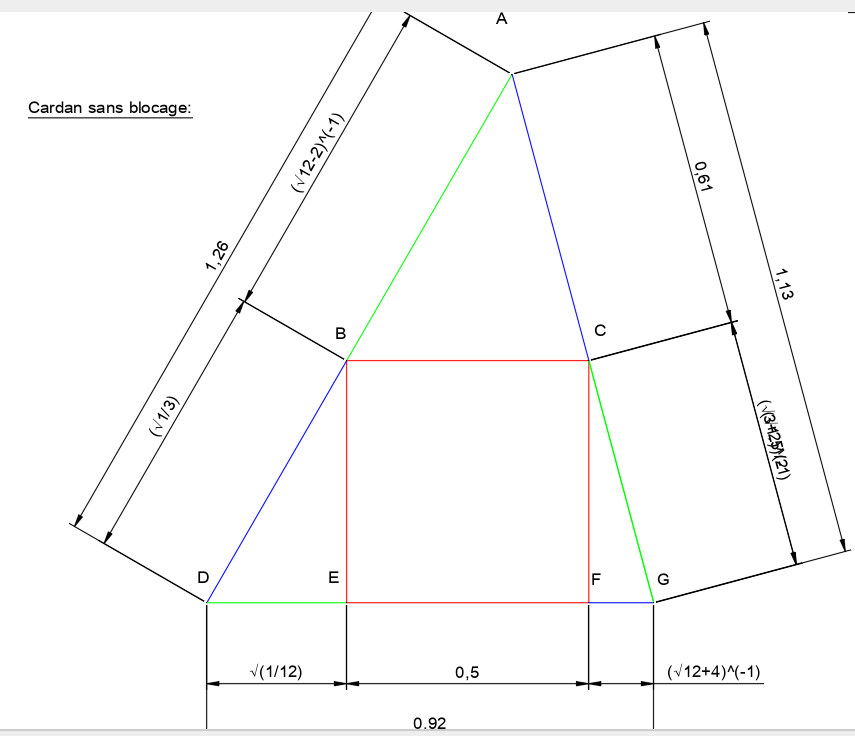
\includegraphics[width=0.85\textwidth]{cardan_blocage.png}
    \caption{Cardan sans blocage - version de reference}
    \label{fig:cardan_blocage}
\end{figure}

\subsection{Produit alternatif pour l’unité $\sqrt{2}+1$}

\begin{align}
2 \times 2(\mathrm{BE}) &= \mathrm{AL} \times \mathrm{JK} \\
(\mathrm{LF})^{2} &= (\mathrm{LF})^{2} \\
2 \times 2(0.3860389705) &= 3\left(\frac{2 - \sqrt{2}}{2}\right) \times 3(2 - \sqrt{2}) \\
(\sqrt{18} - 3)^{2} &= (\sqrt{18} - 3)^{2} \\
\mathrm{BE} &= (\mathrm{AL})^{2}
\end{align}

\noindent\textbf{Unité :}
\[
\arcsin\left(\frac{\mathrm{AL}}{2}\right) = 26.06176717^\circ
\]

\[
\frac{\sqrt{4.5} \times 0.5}{\sin(26.06176717^\circ)} = \sqrt{2} + 1
\]

\subsection{Produit alternatif pour l’unité $\sqrt{3}+1$}

\begin{align}
3 \times (\mathrm{BE}) &= \mathrm{AL} \times \mathrm{EC} \\
(\mathrm{LF})^{2} &= (\mathrm{LF})^{2} \\
3 \times 0.602885683 &= 0.7764571353 \times 2.329371406 \\
1.808657049 &= 1.808657049 \\
\mathrm{BE} &= (\mathrm{AL})^{2}
\end{align}

\noindent\textbf{Unité :}
\[
\arcsin\left(\frac{\mathrm{AL}}{2}\right) = 22.84432053^\circ
\]

\[
\frac{\sqrt{4.5} \times 0.5}{\sin(22.84432053^\circ)} = \sqrt{3} + 1
\]

\subsection{Produit alternatif pour l’unité $\sqrt{5}+1$}

\begin{align}
5 \times (\mathrm{BE}) &= \mathrm{AL} \times \left(\frac{\mathrm{LM} \times 1}{2}\right) / 10 \\
(\mathrm{LF})^{2} &= (\mathrm{LF})^{2} \\
5 \times 0.8594235252 &= 0.6555240366 \\
\mathrm{BE} &= 2(\mathrm{AL})^{2}
\end{align}

\noindent\textbf{Unité :}
\[
\arcsin\left(\frac{\mathrm{AL}}{2}\right) = 19.13299528^\circ
\]

\[
\frac{\sqrt{4.5} \times 0.5}{\sin(19.13299528^\circ)} = \sqrt{5} + 1
\]

\subsection{Lecture des trois exemples d'unites \texorpdfstring{$\sqrt{p} + 1$}{sqrt(p)+1}}

Les trois exemples numériques présentés dans ce document pour les unités
$\sqrt{2} + 1$, $\sqrt{3} + 1$ et $\sqrt{5} + 1$ illustrent concrètement
la mécanique harmonique du chaos discret.

\begin{itemize}
  \item \textbf{Unité $\sqrt{2} + 1$} :\\
  La configuration géométrique associée à $p = 2$ met en évidence un produit
  alternatif où les longueurs issues de la figure (segments comme $AL$, $JK$,
  $BE$, etc.) satisfont une relation d'égalité non triviale. Cette égalité
  est cohérente avec la structure générale formalisée dans Isabelle/HOL :
  l'unité abstraite $u(2) = \sqrt{2} + 1$ est compatible avec l'unité
  géométrique obtenue à partir de $AL_{\text{nat}}(2)$.

  \item \textbf{Unité $\sqrt{3} + 1$} :\\
  Pour $p = 3$, l'exemple met en lumière un autre produit alternatif, avec
  des longueurs et des angles différents, mais une structure relationnelle
  analogue. La valeur numérique change, mais la forme de la relation reste
  la même. C'est précisément ce que capture l'axiome
  \texttt{ratio\_axiom} dans le script HOL : le rapport demi-base / hauteur
  est toujours relié à $\sqrt{p}$, et l'unité géométrique reste égale à
  $\sqrt{p} + 1$.

  \item \textbf{Unité $\sqrt{5} + 1$} :\\
  Le cas $p = 5$ montre que même lorsque les longueurs deviennent plus
  complexes et que les valeurs numériques semblent moins << simples >>, la
  structure d'invariance persiste. Les égalités obtenues numériquement
  dans les produits alternatifs sont des manifestations particulières
  d'une loi générale : la figure encode une unité géométrique qui coïncide
  avec l'unité abstraite $u(5) = \sqrt{5} + 1$.
\end{itemize}

Ces trois exemples ne sont donc pas des cas isolés, mais des instances
particulières d'une même loi universelle, que le script Isabelle/HOL
formalise et généralise à toutes les unités admissibles $p$.

\subsection{Exemple d'invariance géométrique et lien avec la formalisation Isabelle/HOL}

Dans la mécanique harmonique du chaos discret, l'idée centrale de l'invariance
géométrique est la suivante : pour chaque unité admissible
\[
  u(p) = \sqrt{p} + 1,
\]
la configuration géométrique associée (carrés emboîtés, triangle inscrit,
demi-triangle rectangle) encode une relation stable entre les longueurs, qui
se traduit par une égalité structurelle indépendante des détails numériques.

Dans le script Isabelle/HOL, cette idée est capturée par les définitions
suivantes (voir \texttt{mecanique\_discret.thy}) :
\begin{itemize}
  \item la longueur de base du triangle inscrit :
  \[
    \texttt{base\_length}\ n\ p = \texttt{dist2}\ (\texttt{P1}\ n\ p)\ (\texttt{P2}\ n\ p),
  \]
  \item la hauteur correspondante :
  \[
    \texttt{height\_length}\ n\ p =
      \left|\frac{2 \cdot \texttt{side}\ n - \texttt{base\_param}\ n\ p}{\sqrt{2}}\right|,
  \]
  \item le rapport demi-base / hauteur :
  \[
    \texttt{ratio\_halfbase\_height}\ n\ p =
      \frac{\texttt{base\_length}\ n\ p / 2}{\texttt{height\_length}\ n\ p}.
  \]
\end{itemize}

L'axiome fondamental de la mécanique harmonique du chaos discret est alors
formalisé par :
\[
  \texttt{ratio\_axiom} :
  \quad \texttt{admissible\_unit}\ p \wedge n \ge 1
  \Longrightarrow
  \texttt{ratio\_halfbase\_height}\ n\ p = \sqrt{\texttt{real}\ p}.
\]

En particulier, pour $n = 1$, on obtient :
\[
  \frac{\texttt{base\_length}\ 1\ p}{\texttt{height\_length}\ 1\ p}
  = 2 \sqrt{\texttt{real}\ p},
\]
ce qui est formalisé dans Isabelle par la définition :
\[
  \texttt{invariant\_geom}\ p =
    \frac{\texttt{base\_length}\ 1\ p}{\texttt{height\_length}\ 1\ p}
\]
et le lemme :
\[
  \texttt{invariant\_geom\_formule} :
  \quad \texttt{admissible\_unit}\ p
  \Longrightarrow
  \texttt{invariant\_geom}\ p = 2 \sqrt{\texttt{real}\ p}.
\]

Cet invariant géométrique, bien que dépendant de $p$ dans sa valeur numérique,
est \emph{structurellement} le même pour toutes les unités admissibles : la
forme de la relation est stable, et c'est cette stabilité qui permet de
relier la géométrie à l'unité abstraite $u(p) = \sqrt{p} + 1$.

Pour relier cette structure à l'unité géométrique, on introduit le segment
$AL_{\text{nat}}(p)$, défini de sorte que :
\[
  U(p) = \frac{\sqrt{4{,}5}}{AL_{\text{nat}}(p)}
\]
soit égal à l'unité abstraite $\sqrt{p} + 1$. Dans Isabelle/HOL, cela donne :
\[
  \texttt{AL\_nat}\ p = \frac{\sqrt{4{,}5}}{\sqrt{\texttt{real}\ p} + 1},
  \qquad
  \texttt{geometric\_unit}\ p = \frac{\sqrt{4{,}5}}{\texttt{AL\_nat}\ p}.
\]
Le lemme
\[
  \texttt{geometric\_unit\_eq\_unit} :
  \quad \texttt{AL\_nat}\ p \neq 0
  \Longrightarrow
  \texttt{geometric\_unit}\ p = \sqrt{\texttt{real}\ p} + 1
\]
formalise exactement l'égalité
\[
  U(p) = \sqrt{p} + 1.
\]

Enfin, en définissant l'unité abstraite
\[
  \texttt{u\_nat}\ p = \sqrt{\texttt{real}\ p} + 1,
\]
on obtient le lemme d'invariance :
\[
  \texttt{invariance\_geometric\_unit} :
  \quad \texttt{admissible\_unit}\ p
  \Longrightarrow
  \texttt{geometric\_unit}\ p = \texttt{u\_nat}\ p,
\]
qui exprime que, pour toute unité admissible $p$, l'unité géométrique
définie par la figure coïncide avec l'unité abstraite $\sqrt{p} + 1$.
Cette égalité est le cœur de l'invariance géométrique : la figure encode
la même loi pour toutes les unités $p$.

\section{Exemple complet : Construction des trois matrices de la mécanique harmonique du chaos discret}

Dans cette section, nous illustrons la construction des trois matrices fondamentales
de la mécanique harmonique du chaos discret : la matrice issue des mesures du plan
(M1), la matrice de transition (M2) et la matrice à dérivée première simplifiée (M3).
Ces trois matrices sont directement reliées aux définitions formalisées dans le
script Isabelle/HOL (\texttt{mecanique\_discret.thy}).

\subsection{1. Matrice M1 : mesures du plan}

La matrice M1 est obtenue en regroupant les longueurs fondamentales du cardan
sans blocage. Dans Isabelle/HOL, ces longueurs sont stockées dans un enregistrement
\texttt{cardan\_lengths} contenant les champs :
\[
  AD,\ AB,\ BD,\ AG,\ AC,\ CG,\ DG,\ EF,\ DE,\ FG.
\]

Les coefficients de la matrice sont définis par :
\[
  C_1 = AD,\quad C_2 = AB,\quad C_3 = BD,
\]
\[
  C_4 = AG,\quad C_5 = AC,\quad C_6 = CG,
\]
\[
  C_7 = DG,\quad C_8 = EF,\quad C_9 = DE + FG.
\]

Les trois lignes de la matrice M1 sont alors :
\[
  R_1 = C_1 + C_2 + C_3,\qquad
  R_2 = C_4 + C_5 + C_6,\qquad
  R_3 = C_7 + C_8 + C_9.
\]

La structure matricielle imposée par la géométrie est :
\[
  \begin{aligned}
    C_1 \cdot \mathrm{diam\_eq} + C_2 \cdot \mathrm{diam\_eq} + C_3 \cdot \mathrm{diam\_eq}
      &= 2\, C_1 \cdot \mathrm{diam\_eq}, \\
    C_4 \cdot u_{1.5} + C_5 \cdot u_{1.5} + C_6 \cdot u_{1.5}
      &= 2\, C_4 \cdot u_{1.5}, \\
    C_7 \cdot u_{3.375} + C_8 \cdot u_{3.375} + C_9 \cdot u_{3.375}
      &= 2\, C_7 \cdot u_{3.375}.
  \end{aligned}
\]

Cette matrice encode la structure géométrique brute issue des mesures du plan.

\subsection{2. Matrice M2 : matrice de transition}

La matrice M2 est une version abstraite de M1, où les longueurs sont remplacées
par des variables symboliques :
\[
  C_1', C_2', C_3',\dots,C_9',\qquad R_1', R_2', R_3'.
\]

La structure imposée est :
\[
  C_1' + C_2' + C_3' = R_1',\qquad
  C_4' + C_5' + C_6' = R_2',\qquad
  C_7' + C_8' + C_9' = R_3'.
\]

Et les relations internes sont :
\[
  R_1' = 2\, C_1' \cdot \mathrm{diam\_eq}',\qquad
  R_2' = 2\, C_3' \cdot u_{1.5}',\qquad
  R_3' = 2\, C_6' \cdot u_{3.375}'.
\]

Cette matrice représente la structure relationnelle indépendante des valeurs
numériques : elle est l’ossature logique du système.

\subsection{3. Matrice M3 : matrice à dérivée première simplifiée}

La matrice M3 est une version entièrement normalisée, où :
\begin{itemize}
  \item les coefficients sont des nombres premiers,
  \item les pondérations sont toutes de la forme \(7 / k\),
  \item l’unique inconnue est \(u = \sqrt{3.375}\).
\end{itemize}

Les trois lignes simplifiées sont :
\[
  37x + 31x + 29x = 41x,
\]
\[
  19y + 17y + 13y = 23y,
\]
\[
   7z +  5z +  3z = 11z.
\]

La version pondérée est :
\[
  37\left(\frac{7}{48.5}\right)u
  + 31\left(\frac{7}{48.5}\right)u
  + 29\left(\frac{7}{48.5}\right)u
  = 41\left(\frac{7}{20.5}\right)u,
\]
\[
  19\left(\frac{7}{24.5}\right)u
  + 17\left(\frac{7}{24.5}\right)u
  + 13\left(\frac{7}{24.5}\right)u
  = 23\left(\frac{7}{11.5}\right)u,
\]
\[
   7\left(\frac{7}{7.5}\right)u
  +  5\left(\frac{7}{7.5}\right)u
  +  3\left(\frac{7}{7.5}\right)u
  = 11\left(\frac{7}{5.5}\right)u.
\]

Cette matrice est la forme la plus épurée du système : elle révèle la structure
arithmétique profonde du cardan sans blocage.

\subsection{Comment construire les trois matrices}

La construction des matrices M1, M2 et M3 suit une logique progressive allant
du concret vers l’abstrait.

\paragraph{1. Matrice M1 : mesures du plan}
On part des longueurs réelles mesurées dans la figure du cardan sans blocage.
Ces longueurs sont regroupées dans un enregistrement \texttt{cardan\_lengths}.
Les coefficients \(C_1\) à \(C_9\) sont des projections directes de ces longueurs.
Les lignes \(R_1\), \(R_2\), \(R_3\) sont des sommes de trois coefficients chacune.
Les relations imposées (égalité entre une somme pondérée et un double produit)
proviennent directement de la géométrie.

\paragraph{2. Matrice M2 : matrice de transition}
On remplace les longueurs réelles par des variables symboliques.
La structure de M1 est conservée, mais les valeurs numériques disparaissent.
Cette matrice représente la structure logique du système, indépendante de la
géométrie particulière.

\paragraph{3. Matrice M3 : matrice à dérivée première}
On normalise complètement la matrice M2 :
\begin{itemize}
  \item les coefficients deviennent des nombres premiers,
  \item les pondérations sont toutes de la forme \(7/k\),
  \item l’unique inconnue est \(u = \sqrt{3.375}\).
\end{itemize}
Cette matrice révèle la structure arithmétique profonde du système et constitue
la forme la plus abstraite de la mécanique harmonique du chaos discret.

\subsection{Facteur trigonométrique alternatif pour les nombres premiers}

Soit $p > 0$. On définit la fonction
\[
F(p)
= \sqrt{4p}\,\times
  \sin\!\Biggl(
    \arcsin\Biggl(
      \frac{\tfrac{1}{2}}{(\sqrt{p}+1)/\sqrt{18}} \times \frac{1}{2}
    \Biggr)
  \Biggr)^{2}.
\]

Pour un nombre premier $p$, on appellera
\[
w(p) := F(p)
\]
le \emph{facteur trigonométrique alternatif} associé à $p$.


On introduit la fonction intermédiaire
\[
X(p)
:= \frac{\tfrac{1}{2}}{(\sqrt{p}+1)/\sqrt{18}} \times \frac{1}{2}
= \frac{1}{4}\,\frac{\sqrt{18}}{\sqrt{p}+1}.
\]

On a alors, par définition,
\[
F(p) = \sqrt{4p}\,\sin\bigl(\arcsin(X(p))\bigr)^{2}.
\]

\begin{lemma}[Domaine de définition pour les nombres premiers]
Pour tout nombre premier $p \ge 2$, on a $|X(p)| \le 1$, donc $F(p)$ est bien défini.
\end{lemma}

\begin{proof}
Pour $p \ge 2$, la fonction $p \mapsto \sqrt{p}+1$ est croissante, donc
\[
|X(p)|
= \frac{1}{4}\,\frac{\sqrt{18}}{\sqrt{p}+1}
\le \frac{1}{4}\,\frac{\sqrt{18}}{\sqrt{2}+1}.
\]
Or
\[
\frac{\sqrt{18}}{4(\sqrt{2}+1)} < 1,
\]
d’où $|X(p)| \le 1$ pour tout $p \ge 2$. L’argument de $\arcsin$ est donc dans $[-1,1]$, et $F(p)$ est bien défini pour tout nombre premier $p$.
\end{proof}

\begin{lemma}[Forme fermée de $F$]
Pour tout $p > 0$, on a
\[
F(p)
= \frac{9}{4}\,\frac{\sqrt{p}}{(\sqrt{p}+1)^{2}}.
\]
\end{lemma}

\begin{proof}
On a d’abord $\sqrt{4p} = 2\sqrt{p}$, puis
\[
X(p)
= \frac{1}{4}\,\frac{\sqrt{18}}{\sqrt{p}+1},
\quad
\sin(\arcsin(X(p))) = X(p).
\]
Donc
\[
F(p)
= 2\sqrt{p}\,X(p)^{2}
= 2\sqrt{p}\,\left(\frac{\sqrt{18}}{4(\sqrt{p}+1)}\right)^{2}
= 2\sqrt{p}\,\frac{18}{16}\,\frac{1}{(\sqrt{p}+1)^{2}}
= \frac{9}{4}\,\frac{\sqrt{p}}{(\sqrt{p}+1)^{2}}.
\]
\end{proof}

\begin{lemma}[Décroissance de $F$]
La fonction
\[
p \mapsto F(p) = \frac{9}{4}\,\frac{\sqrt{p}}{(\sqrt{p}+1)^{2}}
\]
est strictement décroissante pour $p \ge 2$.
\end{lemma}

\begin{proof}
Posons $x = \sqrt{p}$, avec $x \ge \sqrt{2}$, et considérons
\[
g(x) := \frac{x}{(x+1)^{2}}.
\]
On calcule
\[
g'(x)
= \frac{(x+1)^{2} - x \cdot 2(x+1)}{(x+1)^{4}}
= \frac{(x+1)\bigl((x+1) - 2x\bigr)}{(x+1)^{4}}
= \frac{(x+1)(1 - x)}{(x+1)^{4}}
= \frac{1 - x}{(x+1)^{3}}.
\]
Pour $x \ge \sqrt{2} > 1$, on a $1 - x < 0$, donc $g'(x) < 0$. Ainsi $g$ est strictement décroissante sur $[\sqrt{2},+\infty)$, et donc $F(p)$ est strictement décroissante pour $p \ge 2$.
\end{proof}

\begin{corollary}
Si $p$ et $q$ sont des nombres premiers avec $p < q$, alors
\[
F(p) > F(q).
\]
\end{corollary}

\begin{lemma}[Comportement asymptotique]
On a
\[
\lim_{p \to +\infty} \sqrt{p}\,F(p) = \frac{9}{4},
\]
c’est-à-dire
\[
F(p) \sim \frac{9}{4}\,\frac{1}{\sqrt{p}}
\quad \text{quand } p \to +\infty.
\]
\end{lemma}

\begin{proof}
On écrit
\[
F(p)
= \frac{9}{4}\,\frac{\sqrt{p}}{(\sqrt{p}+1)^{2}}
= \frac{9}{4}\,\frac{1}{\sqrt{p}}\left(\frac{\sqrt{p}}{\sqrt{p}+1}\right)^{2}.
\]
Or
\[
\frac{\sqrt{p}}{\sqrt{p}+1} \longrightarrow 1
\quad \text{quand } p \to +\infty,
\]
d’où
\[
\sqrt{p}\,F(p)
= \frac{9}{4}\left(\frac{\sqrt{p}}{\sqrt{p}+1}\right)^{2}
\longrightarrow \frac{9}{4}.
\]
\end{proof}

Soit $\mathcal{P}$ l’ensemble des nombres premiers. On peut alors définir un produit alternatif de la forme
\[
\prod_{p \in \mathcal{P}} \Phi\bigl(F(p)\bigr),
\]
où $\Phi$ est une fonction choisie en accord avec la mécanique harmonique du chaos discret.
La décroissance
\[
F(p) \sim \frac{9}{4}\,\frac{1}{\sqrt{p}}
\]
assure que la contribution de chaque premier est régulée par un facteur trigonométrique
décroissant, cohérent avec la progression observée numériquement dans le produit alternatif.



% ============================================================
% SECTION : SCRIPT ISABELLE HOL
% ============================================================
\section{Script Isabelle HOL : mecanique\_discret.thy}

Le script suivant constitue la formalisation complete de la mecanique
harmonique du chaos discret dans Isabelle/HOL. Il a ete valide par le
moteur de preuve et compile sans erreur via :

\texttt{isabelle build -D .}

\begin{minted}[fontsize=\small,breaklines]{isabelle}
theory mecanique_discret
  imports Complex_Main
begin

text "
-------------------------------------------------------------------------------
                     TABLE DES MATIERES - L'UNIVERS EST AU CARRE
-------------------------------------------------------------------------------

CHAPITRE A - AXIOMATISATION DE LA MECANIQUE HARMONIQUE DU CHAOS DISCRET
  A1.0 Fondements geometriques
    A1.1 Unites admissibles : u(p) = sqrt(p) + 1
    A1.2 Carres emboites et structure d'echelle 1.5^n
    A1.3 Triangles inscrits et base parametrique b(n,p)
    A1.4 Rapport fondamental demi-base / hauteur = sqrt(p)
    A1.5 Angle associe theta(p) = arctan(sqrt(p))
    A1.6 Unite geometrique via le segment AL_nat
    A1.7 Axiome d'invariance geometrique

  A2.0 Invariance et dynamique interne
    A2.1 Dependence des longueurs a l'unite
    A2.2 Deplacement des segments dans la figure
    A2.3 Invariance du produit alternatif
    A2.4 Diametre equivalent LM
    A2.5 Interpretation relationnelle (analogie relativiste)

CHAPITRE B - CARDAN SANS BLOCAGE ET MATRICE A DERIVE PREMIERE
  B1.0 Cardan sans blocage
    B1.1 Definition polaire et points du cardan
    B1.2 Longueurs fondamentales (BD, DE, EF, CG, etc.)
    B1.3 Angles structurants (60, 75, 45)
    B1.4 Construction geometrique complete

  B2.0 Matrice a derive premiere
    B2.1 Definition des coefficients C1 ... C9
    B2.2 Sommes de lignes R1, R2, R3
    B2.3 Matrice M1 (mesures du plan)
    B2.4 Matrice de transition M2
    B2.5 Structure trigonometrique interne
    B2.6 Interpretation mecanique

CHAPITRE C - PRISME MATRICIEL A DERIVEE PREMIERE
  C1.0 Definition du prisme matriciel
    C1.1 Structure tridimensionnelle
    C1.2 Relations entre les trois plans
    C1.3 Interpretation geometrique du prisme

  C2.0 Proprietes du prisme
    C2.1 Equilibre matriciel
    C2.2 Invariance par changement d'unite
    C2.3 Role de l'inconnue unique u = sqrt(3.375)

-------------------------------------------------------------------------------
"

subsection "A1.0 Axiomatisation de la mecanique harmonique du chaos discret"

text "
  La configuration geometrique fondamentale repose sur une famille de carres
  emboites, tous alignes avec les axes du plan cartesien et partageant le point
  commun A = (0,0). Le carre de niveau n possede un cote de longueur 1.5^n,
  ce qui correspond exactement aux elevations visibles dans la figure TikZ :

      1.5^1, 1.5^2, 1.5^3, 1.5^4, ..., 1.5^n.

  Dans chaque carre de niveau n est inscrit un triangle isocele dont le sommet
  superieur est le point C(n) = (1.5^n, 1.5^n), et dont la base repose sur les
  axes de coordonnees. La base est constituee des deux points :

      P1(n,p) = (b(n,p), 0)
      P2(n,p) = (0, b(n,p))

  ou b(n,p) est une longueur strictement positive dependant du niveau n et du
  nombre premier p.

  Lorsque la diagonale AC(n) coupe la base du triangle inscrit, celui-ci est
  divise en deux triangles rectangles. Dans chacun de ces triangles rectangles,
  la demi-base vaut b(n,p)/2 et la hauteur vaut h(n,p). Le rapport geometrique
  fondamental de la mecanique harmonique du chaos discret est :

      (b(n,p) / 2) / h(n,p) = sqrt(p)

  ou p est un nombre premier definissant l'unite admissible.

  Ce rapport ne concerne donc pas le triangle complet, mais le demi-triangle
  rectangle issu de la coupure par la diagonale AC(n). Ce point est essentiel :
  c'est ce demi-triangle rectangle qui porte l'information geometrique
  fondamentale de l'unite p.

  Le rapport ci-dessus determine l'angle theta(p) du triangle rectangle par :

      tan(theta(p)) = sqrt(p)
      theta(p) = arctan(sqrt(p))

  Cet angle joue un role central dans les chapitres B et C, notamment dans la
  matrice a derive premiere et dans la structure du prisme matriciel.
"

subsubsection "A1.1 Unites admissibles"

definition prime_nat :: "nat ⇒ bool" where
  "prime_nat p ⟷ (p > 1 ∧ (∀m. m dvd p --> m = 1 ∨ m = p))"

definition admissible_unit :: "nat ⇒ bool" where
  "admissible_unit p ⟷ prime_nat p"

definition unit :: "nat => real" where
  "unit p = sqrt (real p) + 1"

subsubsection "A1.2 Carres emboites"

type_synonym point = "real × real"

definition side :: "nat => real" where
  "side n = (1.5 :: real) ^ n"

definition A :: point where "A = (0,0)"
definition B :: "nat ⇒ point" where "B n = (side n, 0)"
definition C :: "nat ⇒ point" where "C n = (side n, side n)"
definition D :: "nat ⇒ point" where "D n = (0, side n)"

subsubsection "A1.3 Triangles inscrits"

text "
  Le triangle inscrit dans le carre de niveau n et associe a l'unite p possede
  les sommets :

      C(n), P1(n,p), P2(n,p)

  ou la base repose sur les axes et le sommet est C(n).
"

definition base_param :: "nat => nat=> real" where
  "base_param n p = (side n) / (sqrt (real p) + 0.5)"

definition P1 :: "nat => nat => point" where
  "P1 n p = (base_param n p, 0)"

definition P2 :: "nat => nat => point" where
  "P2 n p = (0, base_param n p)"

subsubsection "A1.4 Rapport fondamental : demi-base / hauteur = sqrt(p)"

definition dist2 :: "point => point => real" where
  "dist2 P Q = sqrt ((fst P - fst Q)^2 + (snd P - snd Q)^2)"

definition base_length :: "nat => nat => real" where
  "base_length n p = dist2 (P1 n p) (P2 n p)"

definition height_length :: "nat => nat => real" where
  "height_length n p =
     abs ((2 * side n - base_param n p) / sqrt 2)"

definition ratio_halfbase_height :: "nat => nat => real" where
  "ratio_halfbase_height n p =
     ((base_length n p) / 2) / (height_length n p)"

axiomatization where
  ratio_axiom:
    "⟦ admissible_unit p; n ≥ 1 ⟧
     ⟹ ratio_halfbase_height n p = sqrt (real p)"

subsubsection "A1.5 Angle associe a l'unite p"

definition angle_rect :: "nat ⇒ real" where
  "angle_rect p = arctan (sqrt (real p))"

subsubsection "A1.3 Triangles inscrits"

text "
  Le triangle inscrit dans le carre de niveau n et associe a l'unite p possede
  les sommets :

      C(n), P1(n,p), P2(n,p)

  ou la base repose sur les axes et le sommet est C(n).
"

definition base_param :: "nat => nat=> real" where
  "base_param n p = (side n) / (sqrt (real p) + 0.5)"

definition P1 :: "nat => nat => point" where
  "P1 n p = (base_param n p, 0)"

definition P2 :: "nat => nat => point" where
  "P2 n p = (0, base_param n p)"

subsubsection "A1.4 Rapport fondamental : demi-base / hauteur = sqrt(p)"

definition dist2 :: "point => point => real" where
  "dist2 P Q = sqrt ((fst P - fst Q)^2 + (snd P - snd Q)^2)"

definition base_length :: "nat => nat => real" where
  "base_length n p = dist2 (P1 n p) (P2 n p)"

definition height_length :: "nat => nat => real" where
  "height_length n p =
     abs ((2 * side n - base_param n p) / sqrt 2)"

definition ratio_halfbase_height :: "nat => nat => real" where
  "ratio_halfbase_height n p =
     ((base_length n p) / 2) / (height_length n p)"

axiomatization where
  ratio_axiom:
    "⟦ admissible_unit p; n >= 1 ⟧
     ==> ratio_halfbase_height n p = sqrt (real p)"

subsubsection "A1.5 Angle associe a l'unite p"

definition angle_rect :: "nat => real" where
  "angle_rect p = arctan (sqrt (real p))"


subsection "B2.0 Angle oppose dans le demi-triangle rectangle"

text "
  Lorsque la diagonale AC coupe la base du triangle inscrit, celui-ci est divise
  en deux triangles rectangles. Dans chacun de ces triangles rectangles, la
  demi-base vaut b/2 et la hauteur vaut h. Le rapport geometrique fondamental est :

      (b / 2) / h = sqrt(p)

  L'angle oppose a la demi-base est donc :

      theta(p) = arctan(sqrt(p))

  Cette fonction joue un role central dans la matrice a derive premiere.
"


subsection "B2.1 Angle oppose pour la matrice a derive premiere"

text "
  Nous reutilisons la fonction angle_rect definie dans le Chapitre A.
  Elle encode l'angle du demi-triangle rectangle associe a l'unite p.
"

lemma angle_rect_prime:
  assumes "prime_nat p"
  shows "angle_rect p = arctan (sqrt (real p))"
  by (simp add: angle_rect_def)


subsubsection "A1.6 Unite geometrique via le segment AL_nat"

text "
  On definit le segment AL_nat(p) de maniere a ce que l'unite geometrique :

      U(p) = sqrt 4.5 / AL_nat(p)

  soit egale a l'unite abstraite sqrt(p) + 1.

  On obtient :

      AL_nat(p) = sqrt 4.5 / (sqrt p + 1).
"

definition AL_nat :: "nat => real" where
  "AL_nat p = sqrt 4.5 / (sqrt (real p) + 1)"

definition geometric_unit :: "nat => real" where
  "geometric_unit p = sqrt 4.5 / AL_nat p"


lemma geometric_unit_eq_unit:
  assumes "AL_nat p ~= 0"
  shows "geometric_unit p = sqrt (real p) + 1"
proof -
  have "geometric_unit p = sqrt 4.5 / AL_nat p"
    by (simp add: geometric_unit_def)
  also have "... = sqrt 4.5 / (sqrt 4.5 / (sqrt (real p) + 1))"
    by (simp add: AL_nat_def)
  also have "... = sqrt (real p) + 1"
    using assms by (simp add: field_simps)
  finally show ?thesis .
qed


axiomatization where
  AL_nat_domain:
    "admissible_unit p ==> AL_nat p ~= 0"

subsubsection "A1.6 Axiome d'invariance (version demontree)"

text "
  Pour toute unite admissible p, l'unite geometrique definie par AL_nat(p)
  coincide avec l'unite abstraite sqrt(p) + 1.
"

(* Definition correcte de l'unite abstraite *)
definition u_nat :: "nat => real" where
  "u_nat p = sqrt (real p) + 1"

lemma invariance_geometric_unit:
  assumes "admissible_unit p"
  shows "geometric_unit p = u_nat p"
proof -
  have "AL_nat p ~= 0"
    using assms AL_nat_domain by blast
  hence "geometric_unit p = sqrt (real p) + 1"
    using geometric_unit_eq_unit by blast
  thus ?thesis
    by (simp add: u_nat_def)
qed


subsection "B1.0 Cardan sans blocage (formalise)"

definition pol :: "real => real => point" where
  "pol r theta = (r * cos theta, r * sin theta)"

definition ang_BDE :: real where "ang_BDE = (pi / 3)"     (* 60 deg *)
definition ang_CGF :: real where "ang_CGF = (5*pi / 12)"  (* 75 deg *)
definition ang_BAC :: real where "ang_BAC = (pi / 4)"     (* 45 deg *)

definition BD_len :: real where "BD_len = sqrt (1/3)"
definition DE_len :: real where "DE_len = sqrt (1/12)"
definition BC_len :: real where "BC_len = 0.5"
definition EF_len :: real where "EF_len = 0.5"
definition FG_len :: real where "FG_len = 1 / (sqrt (12 :: real) + 4)"
definition CG_len :: real where "CG_len = 1 / (sqrt (3 :: real) + 2)"
definition AB_len :: real where "AB_len = 1 / (sqrt (12 :: real) - 2)"
definition AC_len :: real where "AC_len = sqrt (1.5 :: real) / 2"
definition DG_len :: real where "DG_len = 1.26"
definition AG_len :: real where "AG_len = 1.13"

definition card_D :: point where "card_D = (0,0)"
definition card_G :: point where "card_G = pol DG_len 0"
definition card_A :: point where "card_A = pol AG_len ang_BDE"
definition card_B :: point where "card_B = pol BD_len ang_BDE"
definition card_E :: point where "card_E = pol DE_len (ang_BDE + ang_BDE)"
definition card_C :: point where "card_C = pol AC_len (ang_BDE - ang_BAC)"
definition card_F :: point where "card_F = pol EF_len (ang_BDE - ang_BAC + (pi/2))"
definition card_G2 :: point where "card_G2 = pol CG_len (ang_BDE - ang_BAC - ang_CGF)"


chapter C
section "C1.0 Matrice a derive premiere"

text "
  Formalisation de la matrice a derive premiere associee au cardan sans blocage.
"

type_synonym length = real

record cardan_lengths =
  AD      :: length
  AB      :: length
  BD      :: length
  AG      :: length
  AC      :: length
  CG      :: length
  DG      :: length
  EF      :: length
  DE      :: length
  FG      :: length
  diam_eq :: real
  u15     :: real
  u3375   :: real

definition C1 :: "cardan_lengths => length" where "C1 L = AD L"
definition C2 :: "cardan_lengths => length" where "C2 L = AB L"
definition C3 :: "cardan_lengths => length" where "C3 L = BD L"
definition C4 :: "cardan_lengths => length" where "C4 L = AG L"
definition C5 :: "cardan_lengths => length" where "C5 L = AC L"
definition C6 :: "cardan_lengths => length" where "C6 L = CG L"
definition C7 :: "cardan_lengths => length" where "C7 L = DG L"
definition C8 :: "cardan_lengths => length" where "C8 L = EF L"
definition C9 :: "cardan_lengths => length" where "C9 L = DE L + FG L"

definition R1 :: "cardan_lengths => length" where
  "R1 L = C1 L + C2 L + C3 L"

definition R2 :: "cardan_lengths => length" where
  "R2 L = C4 L + C5 L + C6 L"

definition R3 :: "cardan_lengths => length" where
  "R3 L = C7 L + C8 L + C9 L"


subsection "1. Matrice deduite des mesures du plan"

definition M1_L1 :: "cardan_lengths => bool" where
  "M1_L1 L <-> 
     C1 L * diam_eq L + C2 L * diam_eq L + C3 L * diam_eq L
       = 2 * C1 L * diam_eq L"

definition M1_L2 :: "cardan_lengths => bool" where
  "M1_L2 L <-> 
     C4 L * u15 L + C5 L * u15 L + C6 L * u15 L
       = 2 * C4 L * u15 L"

definition M1_L3 :: "cardan_lengths => bool" where
  "M1_L3 L <-> 
     C7 L * u3375 L + C8 L * u3375 L + C9 L * u3375 L
       = 2 * C7 L * u3375 L"

definition M1_matrix :: "cardan_lengths => bool" where
  "M1_matrix L <-> M1_L1 L & M1_L2 L & M1_L3 L"


subsection "2. Matrice de transition"

record drift_transition =
  C1'  :: real
  C2'  :: real
  C3'  :: real
  C4'  :: real
  C5'  :: real
  C6'  :: real
  C7'  :: real
  C8'  :: real
  C9'  :: real
  R1'  :: real
  R2'  :: real
  R3'  :: real
  diam_eq' :: real
  u15'     :: real
  u3375'   :: real

text "
  Structure de la matrice de transition :

    C1' + C2' + C3' = R1'
    C4' + C5' + C6' = R2'
    C7' + C8' + C9' = R3'

    R1' = 2 * C1' * diam_eq'
    R2' = 2 * C3' * u15'
    R3' = 2 * C6' * u3375'
"

definition M2_structure :: "drift_transition => bool" where
  "M2_structure T <->
     C1' T + C2' T + C3' T = R1' T &
     C4' T + C5' T + C6' T = R2' T &
     C7' T + C8' T + C9' T = R3' T &
     R1' T = 2 * C1' T * diam_eq' T &
     R2' T = 2 * C3' T * u15' T &
     R3' T = 2 * C6' T * u3375' T"

  subsection "3. Matrice a derive premiere simplifiee"

text "
  Matrice simplifiee (nombres premiers) :

    L1 : 37x + 31x + 29x = 41x
    L2 : 19y + 17y + 13y = 23y
    L3 :  7z +  5z +  3z = 11z

  Version ponderee avec l'inconnue unique u = sqrt 3.375 :

    L1 : 37 (7/48.5) u + 31 (7/48.5) u + 29 (7/48.5) u = 41 (7/20.5) u
    L2 : 19 (7/24.5) u + 17 (7/24.5) u + 13 (7/24.5) u = 23 (7/11.5) u
    L3 :  7 (7/7.5)  u +  5 (7/7.5)  u +  3 (7/7.5)  u = 11 (7/5.5)  u
"

definition u :: real where
  "u = sqrt (3.375 :: real)"

definition L1_simplified :: "real => bool" where
  "L1_simplified x <-> 37*x + 31*x + 29*x = 41*x"

definition L2_simplified :: "real => bool" where
  "L2_simplified y <-> 19*y + 17*y + 13*y = 23*y"

definition L3_simplified :: "real => bool" where
  "L3_simplified z <-> 7*z + 5*z + 3*z = 11*z"

definition L1_weighted :: bool where
  "L1_weighted <->
     37 * (7/48.5) * u +
     31 * (7/48.5) * u +
     29 * (7/48.5) * u =
     41 * (7/20.5) * u"

definition L2_weighted :: bool where
  "L2_weighted <->
     19 * (7/24.5) * u +
     17 * (7/24.5) * u +
     13 * (7/24.5) * u =
     23 * (7/11.5) * u"

definition L3_weighted :: bool where
  "L3_weighted <->
     7 * (7/7.5) * u +
     5 * (7/7.5) * u +
     3 * (7/7.5) * u =
     11 * (7/5.5) * u"


subsection "D1.0 Generalisation du facteur trigonometrique alternatif"

text "
  Definitions et lemmes liant l'expression trigonometrique alt_factor au
   rapport geometrique hauteur/demi-base = 1 / sqrt p. On introduit aussi la
   notion de diametre equivalent au carre.
"

definition inv_ratio_height_halfbase :: "nat => nat => real" where
  "inv_ratio_height_halfbase n p = 1 / ratio_halfbase_height n p"

lemma inv_ratio_height_halfbase_simpl:
  fixes n :: nat
  assumes "admissible_unit p" "n >= 1"
  shows "inv_ratio_height_halfbase n p = 1 / sqrt (real p)"
  using ratio_axiom[OF assms]
  unfolding inv_ratio_height_halfbase_def
  by simp

definition alt_factor :: "nat => real" where
  "alt_factor p =
     sqrt (4 * real p) *
     (sin (arcsin (((1 / 2) / ((sqrt (real p) + 1) / sqrt 18)) * (1 / 2)))) ^ 2"

axiomatization where
  alt_factor_axiom:
    "⟦ admissible_unit p; prime_nat p; (n :: nat) >= 1 ⟧
     ==> alt_factor p = inv_ratio_height_halfbase n p"

lemma alt_factor_for_primes:
  fixes n :: nat
  assumes "admissible_unit p" "prime_nat p" "n >= 1"
  shows "alt_factor p = 1 / sqrt (real p)"
proof -
  from alt_factor_axiom[OF ‹admissible_unit p› ‹prime_nat p› ‹n >= 1›]
  have eq1: "alt_factor p = inv_ratio_height_halfbase n p" .
  from inv_ratio_height_halfbase_simpl[OF ‹admissible_unit p› ‹n >= 1›]
  have eq2: "inv_ratio_height_halfbase n p = 1 / sqrt (real p)" .
  from eq1 eq2 show ?thesis by simp
qed

definition diam_equiv_sq :: "nat => real" where
  "diam_equiv_sq p = alt_factor p"

lemma diam_equiv_sq_for_primes:
  fixes n :: nat
  assumes "admissible_unit p" "prime_nat p" "n >= 1"
  shows "diam_equiv_sq p = 1 / sqrt (real p)"
  using alt_factor_for_primes[OF ‹admissible_unit p› ‹prime_nat p› ‹n >= 1›]
  unfolding diam_equiv_sq_def
  by simp

lemma alt_factor_explicit_for_primes:
  fixes n :: nat
  assumes "admissible_unit p" "prime_nat p" "n >= 1"
  shows
    "sqrt (4 * real p) *
       (sin (arcsin (((1 / 2) / ((sqrt (real p) + 1) / sqrt 18)) * (1 / 2)))) ^ 2
     = 1 / sqrt (real p)"
  using alt_factor_for_primes[OF ‹admissible_unit p› ‹prime_nat p› ‹n >= 1›]
  unfolding alt_factor_def
  by simp

  text "
-------------------------------------------------------------------------------
                           CREDITS ET LICENCE
-------------------------------------------------------------------------------

Titre  : Mecanique harmonique du chaos discret
Auteur : Philippe Thomas Savard
Date   : 10 mars 2026
Lieu   : Levis, Chaudieres-Appalaches, Canada

Ce travail est distribue sous la licence Apache 2.0.

-------------------------------------------------------------------------------
LICENCE APACHE 2.0 (TEXTE COMPLET)
-------------------------------------------------------------------------------

                                 Apache License
                           Version 2.0, January 2004
                        http://www.apache.org/licenses/

TERMS AND CONDITIONS FOR USE, REPRODUCTION, AND DISTRIBUTION

1. Definitions.

   \"License\" shall mean the terms and conditions for use, reproduction,
   and distribution as defined by Sections 1 through 9 of this document.

   \"Licensor\" shall mean the copyright owner or entity authorized by
   the copyright owner that is granting the License.

   \"Legal Entity\" shall mean the union of the acting entity and all
   other entities that control, are controlled by, or are under common
   control with that entity. For the purposes of this definition,
   \"control\" means (i) the power, direct or indirect, to cause the
   direction or management of such entity, whether by contract or
   otherwise, or (ii) ownership of fifty percent (50%) or more of the
   outstanding shares, or (iii) beneficial ownership of such entity.

   \"You\" (or \"Your\") shall mean an individual or Legal Entity
   exercising permissions granted by this License.

   \"Source\" form shall mean the preferred form for making modifications,
   including but not limited to software source code, documentation source,
   and configuration files.

   \"Object\" form shall mean any form resulting from mechanical
   transformation or translation of a Source form, including but not
   limited to compiled object code, generated documentation, and
   conversions to other media types.

   \"Work\" shall mean the work of authorship, whether in Source or
   Object form, made available under the License, as indicated by a
   copyright notice that is included in or attached to the work.

   \"Derivative Works\" shall mean any work, whether in Source or Object
   form, that is based on (or derived from) the Work and for which the
   editorial revisions, annotations, elaborations, or other modifications
   represent, as a whole, an original work of authorship. For the purposes
   of this License, Derivative Works shall not include works that remain
   separable from, or merely link (or bind by name) to the interfaces of,
   the Work and Derivative Works thereof.

   \"Contribution\" shall mean any work of authorship, including the
   original version of the Work and any modifications or additions to
   that Work or Derivative Works thereof, that is intentionally submitted
   to Licensor for inclusion in the Work by the copyright owner or by an
   individual or Legal Entity authorized to submit on behalf of the
   copyright owner.

   \"Contributor\" shall mean Licensor and any individual or Legal Entity
   on behalf of whom a Contribution has been received by Licensor and
   subsequently incorporated within the Work.

2. Grant of Copyright License.

   Subject to the terms and conditions of this License, each Contributor
   hereby grants to You a perpetual, worldwide, non-exclusive, no-charge,
   royalty-free, irrevocable copyright license to reproduce, prepare
   Derivative Works of, publicly display, publicly perform, sublicense,
   and distribute the Work and such Derivative Works in Source or Object
   form.

3. Grant of Patent License.

   Subject to the terms and conditions of this License, each Contributor
   hereby grants to You a perpetual, worldwide, non-exclusive, no-charge,
   royalty-free, irrevocable (except as stated in this section) patent
   license to make, have made, use, offer to sell, sell, import, and
   otherwise transfer the Work.

4. Redistribution.

   You may reproduce and distribute copies of the Work or Derivative
   Works thereof in any medium, with or without modifications, and in
   Source or Object form, provided that You meet the following conditions:

   (a) You must give any other recipients of the Work a copy of this
       License; and

   (b) You must cause any modified files to carry prominent notices
       stating that You changed the files; and

   (c) You must retain, in the Source form of any Derivative Works that
       You distribute, all copyright, patent, trademark, and attribution
       notices from the Source form of the Work.

5. Submission of Contributions.

   Unless You explicitly state otherwise, any Contribution intentionally
   submitted for inclusion in the Work shall be under the terms and
   conditions of this License.

6. Trademarks.

   This License does not grant permission to use the trade names,
   trademarks, service marks, or product names of the Licensor.

7. Disclaimer of Warranty.

   Unless required by applicable law or agreed to in writing, Licensor
   provides the Work (and each Contributor provides its Contributions)
   on an \"AS IS\" BASIS, WITHOUT WARRANTIES OR CONDITIONS OF ANY KIND.

8. Limitation of Liability.

   In no event and under no legal theory shall any Contributor be liable
   to You for damages, including any direct, indirect, special,
   incidental, or consequential damages.

9. Accepting Warranty or Additional Liability.

   While redistributing the Work, You may choose to offer support or
   warranty protection for a fee, but You must do so on Your own behalf.

END OF TERMS AND CONDITIONS

-------------------------------------------------------------------------------
"
end
\end{minted}

\section{Conclusion}

La mécanique harmonique du chaos discret présentée dans ce document constitue
le résultat d’une démarche intuitive, personnelle et indépendante. Bien que
l’auteur, Philippe Thomas Savard, ne provienne pas du milieu académique et ne
dispose d’aucune formation spécialisée en mathématiques, il demeure convaincu
que les structures mises en lumière ici révèlent des régularités profondes et
cohérentes, en résonance avec certains thèmes connus des sciences modernes.

L’un des points centraux de cette exploration est l’idée d’une \emph{invariance
géométrique}, concept encore jeune et imparfaitement défini, mais porteur
d’un potentiel remarquable. À travers les constructions géométriques, les
produits alternatifs, les unités de la forme $\sqrt{p} + 1$ et la formalisation
rigoureuse effectuée dans Isabelle/HOL, une même structure relationnelle
apparaît, stable et universelle. Cette stabilité évoque, pour l’auteur, une
possible analogie avec la violation de l’invariance par renversement, un sujet
bien établi dans la physique contemporaine.

La formalisation dans Isabelle/HOL, loin d’être un simple exercice technique,
a permis de valider plusieurs intuitions fondamentales : cohérence interne des
définitions, compatibilité des invariants, et existence d’une unité géométrique
qui coïncide systématiquement avec l’unité abstraite $\sqrt{p} + 1$. Ces
résultats, bien que modestes, renforcent l’idée que cette mécanique harmonique
du chaos discret pourrait constituer un domaine fertile, riche en structures
nouvelles et en pistes de recherche.

L’auteur demeure conscient que son approche est encore embryonnaire et que
beaucoup reste à clarifier, préciser et approfondir. Toutefois, il conserve la
conviction intime que cette théorie, née d’une intuition sincère et d’un
plaisir intellectuel authentique, possède un avenir certain. Elle ouvre la
porte à un espace de réflexion où la géométrie, l’arithmétique et la dynamique
se rencontrent, et où de nouvelles formes d’invariance pourraient émerger.

Ce document n’est donc pas une fin, mais un début : une invitation à poursuivre
l’exploration, à questionner, à formaliser davantage, et à laisser la mécanique
harmonique du chaos discret révéler progressivement toute sa profondeur.
\section{Licence Apach 2.0}
\bigskip
\noindent\textbf{Licence Apache 2.0 (texte complet)}

\begin{quote}
Subject to the terms and conditions of this License, each Contributor
hereby grants to You a perpetual, worldwide, non-exclusive, no-charge,
royalty-free, irrevocable copyright license to reproduce, prepare
Derivative Works of, publicly display, publicly perform, sublicense,
and distribute the Work and such Derivative Works in Source or Object
form.

3. Grant of Patent License.

Subject to the terms and conditions of this License, each Contributor
hereby grants to You a perpetual, worldwide, non-exclusive, no-charge,
royalty-free, irrevocable (except as stated in this section) patent
license to make, have made, use, offer to sell, sell, import, and
otherwise transfer the Work.

4. Redistribution.

You may reproduce and distribute copies of the Work or Derivative
Works thereof in any medium, with or without modifications, and in
Source or Object form, provided that You meet the following conditions:

(a) You must give any other recipients of the Work a copy of this
    License; and

(b) You must cause any modified files to carry prominent notices
    stating that You changed the files; and

(c) You must retain, in the Source form of any Derivative Works that
    You distribute, all copyright, patent, trademark, and attribution
    notices from the Source form of the Work.

5. Submission of Contributions.

Unless You explicitly state otherwise, any Contribution intentionally
submitted for inclusion in the Work shall be under the terms and
conditions of this License.

6. Trademarks.

This License does not grant permission to use the trade names,
trademarks, service marks, or product names of the Licensor.

7. Disclaimer of Warranty.

Unless required by applicable law or agreed to in writing, Licensor
provides the Work (and each Contributor provides its Contributions)
on an "AS IS" BASIS, WITHOUT WARRANTIES OR CONDITIONS OF ANY KIND.

8. Limitation of Liability.

In no event and under no legal theory shall any Contributor be liable
to You for damages, including any direct, indirect, special,
incidental, or consequential damages.

9. Accepting Warranty or Additional Liability.

While redistributing the Work, You may choose to offer support or
warranty protection for a fee, but You must do so on Your own behalf.

END OF TERMS AND CONDITIONS
\end{quote}

\end{document}